\documentclass{ximera}

 

\usepackage{epsfig}

\graphicspath{
  {./}
  {figures/}
}

\usepackage{morewrites}
\makeatletter
\newcommand\subfile[1]{%
\renewcommand{\input}[1]{}%
\begingroup\skip@preamble\otherinput{#1}\endgroup\par\vspace{\topsep}
\let\input\otherinput}
\makeatother

\newcommand{\includeexercises}{\directlua{dofile("/home/jim/linearAlgebra/laode/exercises.lua")}}

%\newcounter{ccounter}
%\setcounter{ccounter}{1}
%\newcommand{\Chapter}[1]{\setcounter{chapter}{\arabic{ccounter}}\chapter{#1}\addtocounter{ccounter}{1}}

%\newcommand{\section}[1]{\section{#1}\setcounter{thm}{0}\setcounter{equation}{0}}

%\renewcommand{\theequation}{\arabic{chapter}.\arabic{section}.\arabic{equation}}
%\renewcommand{\thefigure}{\arabic{chapter}.\arabic{figure}}
%\renewcommand{\thetable}{\arabic{chapter}.\arabic{table}}

%\newcommand{\Sec}[2]{\section{#1}\markright{\arabic{ccounter}.\arabic{section}.#2}\setcounter{equation}{0}\setcounter{thm}{0}\setcounter{figure}{0}}

\newcommand{\Sec}[2]{\section{#1}}

\setcounter{secnumdepth}{2}
%\setcounter{secnumdepth}{1} 

%\newcounter{THM}
%\renewcommand{\theTHM}{\arabic{chapter}.\arabic{section}}

\newcommand{\trademark}{{R\!\!\!\!\!\bigcirc}}
%\newtheorem{exercise}{}

\newcommand{\dfield}{{\sf dfield9}}
\newcommand{\pplane}{{\sf pplane9}}

\newcommand{\EXER}{\section*{Exercises}}%\vspace*{0.2in}\hrule\small\setcounter{exercise}{0}}
\newcommand{\CEXER}{}%\vspace{0.08in}\begin{center}Computer Exercises\end{center}}
\newcommand{\TEXER}{} %\vspace{0.08in}\begin{center}Hand Exercises\end{center}}
\newcommand{\AEXER}{} %\vspace{0.08in}\begin{center}Hand Exercises\end{center}}

% BADBAD: \newcommand{\Bbb}{\bf}

\newcommand{\R}{\mbox{$\Bbb{R}$}}
\newcommand{\C}{\mbox{$\Bbb{C}$}}
\newcommand{\Z}{\mbox{$\Bbb{Z}$}}
\newcommand{\N}{\mbox{$\Bbb{N}$}}
\newcommand{\D}{\mbox{{\bf D}}}
\usepackage{amssymb}
%\newcommand{\qed}{\hfill\mbox{\raggedright$\square$} \vspace{1ex}}
%\newcommand{\proof}{\noindent {\bf Proof:} \hspace{0.1in}}

\newcommand{\setmin}{\;\mbox{--}\;}
\newcommand{\Matlab}{{M\small{AT\-LAB}} }
\newcommand{\Matlabp}{{M\small{AT\-LAB}}}
\newcommand{\computer}{\Matlab Instructions}
\newcommand{\half}{\mbox{$\frac{1}{2}$}}
\newcommand{\compose}{\raisebox{.15ex}{\mbox{{\scriptsize$\circ$}}}}
\newcommand{\AND}{\quad\mbox{and}\quad}
\newcommand{\vect}[2]{\left(\begin{array}{c} #1_1 \\ \vdots \\
 #1_{#2}\end{array}\right)}
\newcommand{\mattwo}[4]{\left(\begin{array}{rr} #1 & #2\\ #3
&#4\end{array}\right)}
\newcommand{\mattwoc}[4]{\left(\begin{array}{cc} #1 & #2\\ #3
&#4\end{array}\right)}
\newcommand{\vectwo}[2]{\left(\begin{array}{r} #1 \\ #2\end{array}\right)}
\newcommand{\vectwoc}[2]{\left(\begin{array}{c} #1 \\ #2\end{array}\right)}

\newcommand{\ignore}[1]{}


\newcommand{\inv}{^{-1}}
\newcommand{\CC}{{\cal C}}
\newcommand{\CCone}{\CC^1}
\newcommand{\Span}{{\rm span}}
\newcommand{\rank}{{\rm rank}}
\newcommand{\trace}{{\rm tr}}
\newcommand{\RE}{{\rm Re}}
\newcommand{\IM}{{\rm Im}}
\newcommand{\nulls}{{\rm null\;space}}

\newcommand{\dps}{\displaystyle}
\newcommand{\arraystart}{\renewcommand{\arraystretch}{1.8}}
\newcommand{\arrayfinish}{\renewcommand{\arraystretch}{1.2}}
\newcommand{\Start}[1]{\vspace{0.08in}\noindent {\bf Section~\ref{#1}}}
\newcommand{\exer}[1]{\noindent {\bf \ref{#1}}}
\newcommand{\ans}{}
\newcommand{\matthree}[9]{\left(\begin{array}{rrr} #1 & #2 & #3 \\ #4 & #5 & #6
\\ #7 & #8 & #9\end{array}\right)}
\newcommand{\cvectwo}[2]{\left(\begin{array}{c} #1 \\ #2\end{array}\right)}
\newcommand{\cmatthree}[9]{\left(\begin{array}{ccc} #1 & #2 & #3 \\ #4 & #5 &
#6 \\ #7 & #8 & #9\end{array}\right)}
\newcommand{\vecthree}[3]{\left(\begin{array}{r} #1 \\ #2 \\
#3\end{array}\right)}
\newcommand{\cvecthree}[3]{\left(\begin{array}{c} #1 \\ #2 \\
#3\end{array}\right)}
\newcommand{\cmattwo}[4]{\left(\begin{array}{cc} #1 & #2\\ #3
&#4\end{array}\right)}

\newcommand{\Matrix}[1]{\ensuremath{\left(\begin{array}{rrrrrrrrrrrrrrrrrr} #1 \end{array}\right)}}

\newcommand{\Matrixc}[1]{\ensuremath{\left(\begin{array}{cccccccccccc} #1 \end{array}\right)}}



\renewcommand{\labelenumi}{\theenumi)}
\newenvironment{enumeratea}%
{\begingroup
 \renewcommand{\theenumi}{\alph{enumi}}
 \renewcommand{\labelenumi}{(\theenumi)}
 \begin{enumerate}}
 {\end{enumerate}\endgroup}



\newcounter{help}
\renewcommand{\thehelp}{\thesection.\arabic{equation}}

%\newenvironment{equation*}%
%{\renewcommand\endequation{\eqno (\theequation)* $$}%
%   \begin{equation}}%
%   {\end{equation}\renewcommand\endequation{\eqno \@eqnnum
%$$\global\@ignoretrue}}

%\input{psfig.tex}

\author{Martin Golubitsky and Michael Dellnitz}

%\newenvironment{matlabEquation}%
%{\renewcommand\endequation{\eqno (\theequation*) $$}%
%   \begin{equation}}%
%   {\end{equation}\renewcommand\endequation{\eqno \@eqnnum
% $$\global\@ignoretrue}}

\newcommand{\soln}{\textbf{Solution:} }
\newcommand{\exercap}[1]{\centerline{Figure~\ref{#1}}}
\newcommand{\exercaptwo}[1]{\centerline{Figure~\ref{#1}a\hspace{2.1in}
Figure~\ref{#1}b}}
\newcommand{\exercapthree}[1]{\centerline{Figure~\ref{#1}a\hspace{1.2in}
Figure~\ref{#1}b\hspace{1.2in}Figure~\ref{#1}c}}
\newcommand{\para}{\hspace{0.4in}}

\renewenvironment{solution}{\suppress}{\endsuppress}

\ifxake
\newenvironment{matlabEquation}{\begin{equation}}{\end{equation}}
\else
\newenvironment{matlabEquation}%
{\let\oldtheequation\theequation\renewcommand{\theequation}{\oldtheequation*}\begin{equation}}%
  {\end{equation}\let\theequation\oldtheequation}
\fi

\makeatother


\title{Least Squares Fitting of Data}

\begin{document}
\begin{abstract}
\end{abstract}
\maketitle

 \label{S:7.6}
\index{least squares!fitting of data}
\index{fitting of data}

We begin this section by using the method of least squares to find the
best straight line fit to a set of data.  Later in the section we will
discuss best fits to other curves.

\subsubsection*{An Example of Best Linear Fit to Data}
\index{linear!fit to data}

Suppose that we are given $n$ data points\index{data points}
$(x_i,y_i)$ for $i=1,\ldots,10$.
For example, consider the ten points
\begin{matlabEquation}  \label{E:scatterdata}
\begin{array}{ccccc}
(2.0,0.1) & (3.0,2.7) & (1.5,-1.1) & (-1.0,-5.5) & (0.0,-3.4)\\
(3.6,3.0) & (0.7,-2.8) & (4.1,4.0) & (1.9,-1.9) & (5.0,5.5) \end{array}
\end{matlabEquation}
The ten points $(x_i,y_i)$ are plotted in Figure~\ref{F:linreg} using the
commands
\begin{verbatim}
e10_3_1
plot(X,Y,'o')
axis([-3,7,-8,8])
xlabel('x')
ylabel('y')
\end{verbatim}
\begin{figure}[htb]
     \centerline{%
     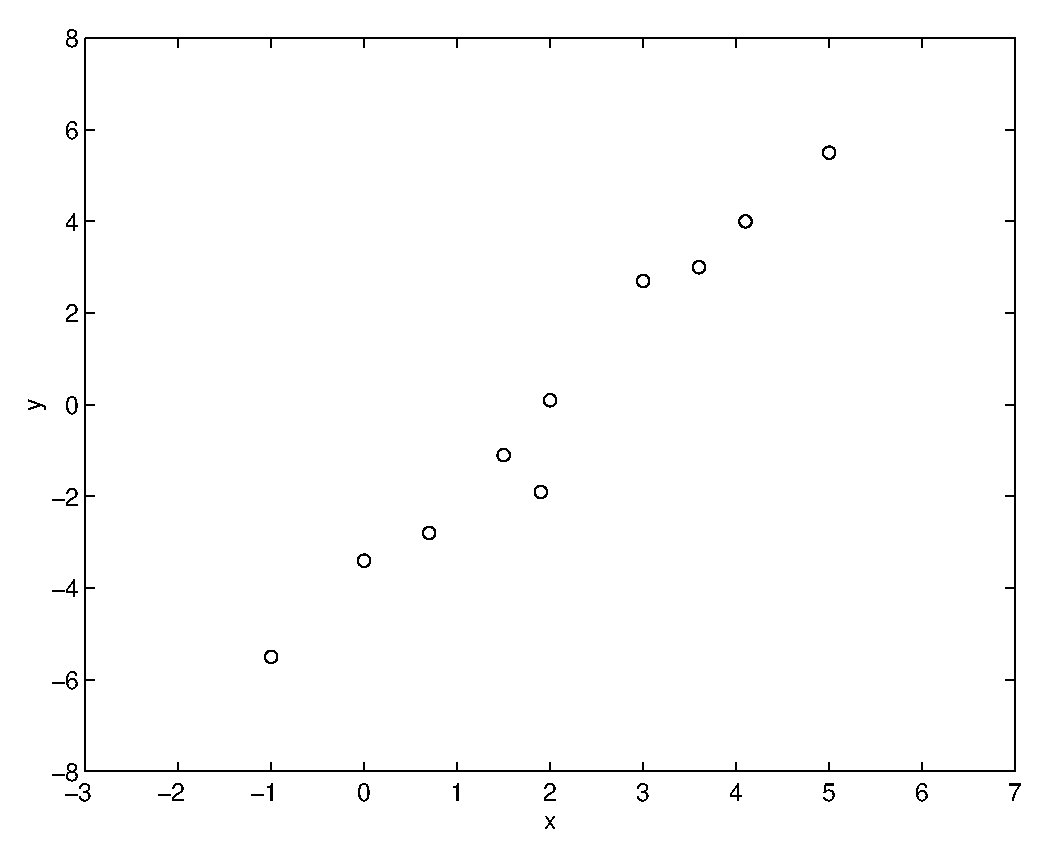
\psfig{file=../figures/linreg.eps,width=2.5in}}
     \caption{Scatter plot of data in \protect\eqref{E:scatterdata}.}
     \label{F:linreg}
\end{figure}

Next, suppose that there is a linear relation between the $x_i$ and the $y_i$;
that is, we assume that there are constants $b_1$ and $b_2$ (that do not
depend on $i$) for which $y_i=b_1+b_2x_i$ for each $i$. But these points are
just data; errors may have been made in their measurement.  So we ask:  Find
$b_1^0$ and $b_2^0$ so that the error made in fitting the data to the line
$y=b_1^0+b_2^0x$ is minimal, that is, the error that is made in that fit is
less than or equal to the error made in fitting the data to the line
$y=b_1+b_2x$ for any other choice of $b_1$ and $b_2$.

We begin by discussing what that error actually is.  Given constants $b_1$ and
$b_2$ and given a data point $x_i$, the difference between the
data value\index{data value}
$y_i$ and the hypothesized value $b_1+b_2x_i$ is the error that is made at that
data point.  Next, we combine the errors made at all of the data points; a
standard way to combine the errors is to use the
Euclidean distance\index{distance!Euclidean}
\[
E(b) =
\left((y_1-(b_1+b_2x_1))^2+\cdots+(y_{10}-(b_1+b_2x_{10}))^2\right)^{\half}.
\]
Rewriting $E(b)$ in vector notation leads to an economy in notation and
to a conceptual advantage.  Let
\[
X=(x_1,\ldots,x_{10})^t \quad Y=(y_1,\ldots,y_{10})^t \AND
F_1=(1,1,\ldots,1)
\]
be vectors in $\R^{10}$.  Then in coordinates
\[
Y-(b_1F_1+b_2X) = \left(\begin{array}{c} y_1-(b_1+b_2x_1)\\ \vdots\\
y_{10}-(b_1+b_2x_{10})\end{array}\right).
\]
It follows that
\[
E(b) = ||Y-(b_1F_1+b_2X)||.
\]
The problem of making a least squares fit is to minimize $E$ over all $b_1$
and $b_2$.

To solve the minimization problem\index{minimization problem},
note that the vectors $b_1F_1+b_2X$ form
a two dimensional subspace $W=\Span\{F_1,X\}\subset\R^{10}$
\index{span} (at least when $X$
is not a scalar multiple of $F_1$, which is almost always).  Minimizing $E$ is
identical to finding a vector $w_0=b_1^0F_1+b_2^0X\in W$ that is nearest to
the vector $Y\in\R^{10}$.   This is the
least squares\index{least squares} question that we solved
in the Section~\ref{S:LSA}.

We can use \Matlab to compute the values of $b_1^0$ and $b_2^0$ that give the
best linear approximation to $Y$.  If we set the matrix $A=(F_1|X)$, then
Theorem~\ref{T:nearestvector} implies that the values of $b_1^0$ and $b_2^0$
are obtained using \eqref{E:nearestvector}.  In particular, type {\tt e10\_3\_1}
to call the vectors {\tt X, Y, F1} into \Matlabp, and then type
\begin{verbatim}
A = [F1 X];
b0 = inv(A'*A)*A'*Y
\end{verbatim}
to obtain
\begin{verbatim}
b0(1) = -3.8597
b0(2) =  1.8845
\end{verbatim}
Superimposing the line $y=-3.8597+1.8845x$ on the
scatter plot\index{scatter plot} in
Figure~\ref{F:linreg} yields the plot in Figure~\ref{F:linreg2}.
The total error is $E(b0)=1.9634$ (obtained in \Matlab by typing
{\tt norm(Y-(b0(1)*F1+b0(2)*X)})\index{\computer!norm}.
Compare this with the error
$E(2,-4)=2.0928$.
\begin{figure}[htb]
     \centerline{%
     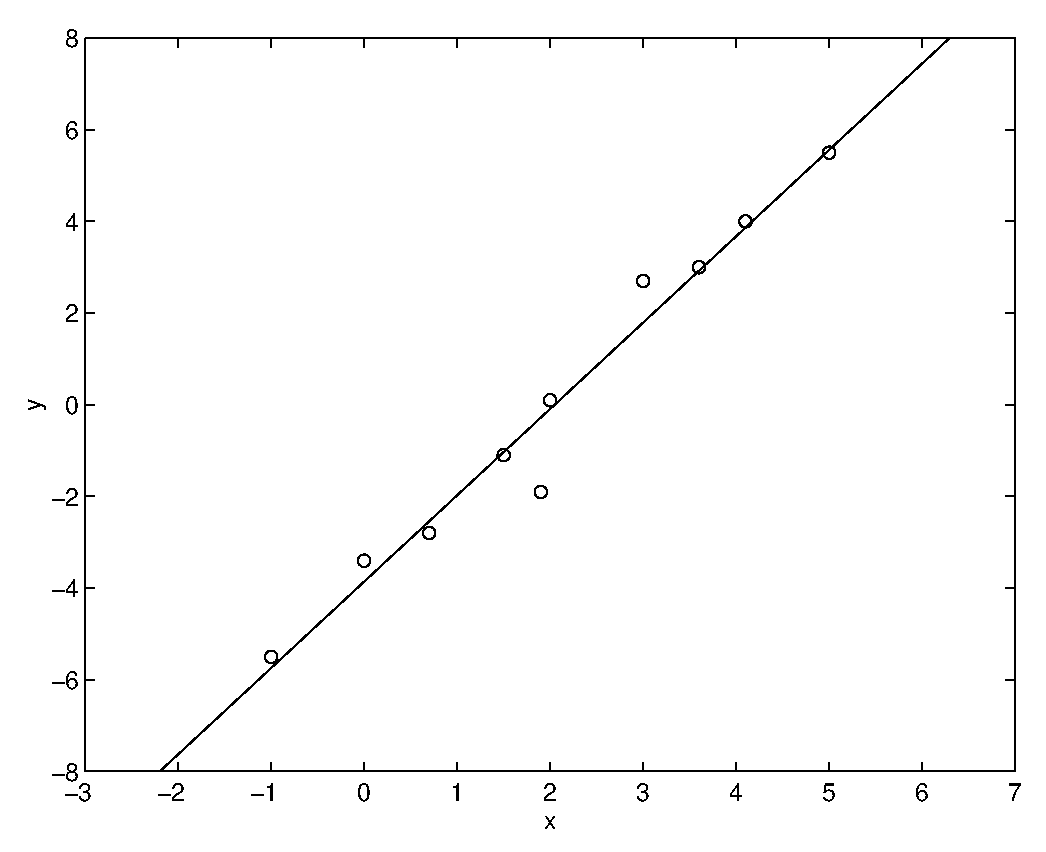
\psfig{file=../figures/linreg2.eps,width=2.5in}}
     \caption{Scatter plot of data in \protect\eqref{E:scatterdata} with best
	linear approximation.}
     \label{F:linreg2}
\end{figure}

\subsubsection*{General Linear Regression}
\index{linear!regression}

We can summarize the previous discussion, as follows.  Given $n$ data points
\[
(x_1,y_1),\ldots, (x_n,y_n);
\]
form the vectors
\[
X=(x_1,\ldots,x_n)^t \quad Y=(y_1,\ldots,y_n)^t \AND F_1=(1,\ldots,1)^t
\]
in $\R^n$.  Find constants $b_1^0$ and $b_2^0$ so that $b_1^0F_1+b_2^0X$ is
a vector in $W=\Span\{F_1,X\}\subset\R^n$ that is nearest to $Y$.  Let
\[
A=(F_1|X)
\]
be the $n\times 2$ matrix.  This problem is solved by least squares in
\eqref{E:nearestvector} as
\begin{equation}  \label{E:LSlinfit}
\vectwo{b_1^0}{b_2^0} = (A^tA)\inv A^tY.
\end{equation}


\subsection*{Least Squares Fit to a Quadratic Polynomial}
\index{least squares!fit to a quadratic polynomial}

Suppose that we want to fit the data $(x_i,y_i)$ to a quadratic polynomial
\[
y=b_1+b_2x+b_3x^2
\]
by least squares methods.  We want to find constants $b_1^0,b_2^0,b_3^0$ so
that the error made is using the quadratic polynomial $y=b_1^0+b_2^0x+b_3^0x^2$
is minimal among all possible choices of quadratic polynomials.  The least
squares error is
\[
E(b) = ||Y-\left(b_1F_1+b_2X+b_3X^{(2)}\right)||
\]
where
\[
X^{(2)}=\left(x_1^2,\ldots,x_n^2\right)^t
\]
and, as before, $F_1$ is the $n$ vector with all components equal to $1$.

We solve the minimization problem as before.  In this case, the space of
possible approximations to the data $W$ is three dimensional; indeed,
$W=\Span\{F_1,X,X^{(2)}\}$.  As in the case of fits to lines we try to
find a point in $W$ that is nearest to the vector $Y\in\R^n$.  By
\eqref{E:nearestvector}, the answer is:
\[
b = (A^tA)\inv A^tY,
\]
where $A=(F_1|X|X^{(2)})$ is an $n\times 3$ matrix.

Suppose that we try to fit the data in \eqref{E:scatterdata} with a quadratic
polynomial rather than a linear one.   Use \Matlab as follows
\begin{verbatim}
e10_3_1
A = [F1 X X.*X];
b = inv(A'*A)*A'*Y;
\end{verbatim}
to obtain
\begin{verbatim}
b0(1) =   0.0443
b0(2) =   1.7054
b0(3) =  -3.8197
\end{verbatim}
So the best parabolic fit\index{parabolic fit}
to this data is $y=-3.8197+1.7054x+0.0443x^2$.
Note that the coefficient of $x^2$ is small suggesting that the data was
well fit by a straight line.  Note also that the error is
$E(b0)=1.9098$ which
is only marginally smaller than the error for the best linear fit.  For
comparison, in Figure~\ref{F:linreg3} we superimpose the equation for the
quadratic fit onto Figure~\ref{F:linreg2}.
\begin{figure}[htb]
     \centerline{%
     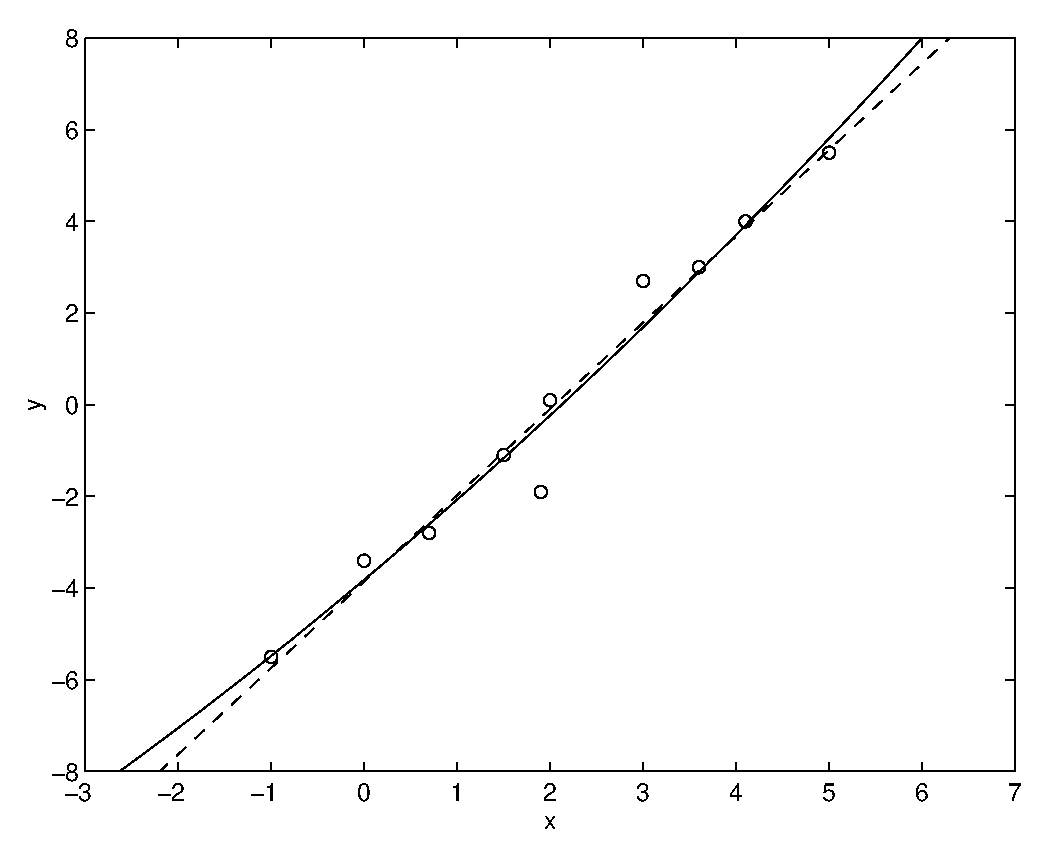
\psfig{file=../figures/linreg3.eps,width=2.5in}}
     \caption{Scatter plot of data in \protect\eqref{E:scatterdata} with best
	linear and quadratic approximations.  The best linear fit is plotted
	with a dashed line.}
     \label{F:linreg3}
\end{figure}\index{scatter plot}



\subsection*{General Least Squares Fit}
\index{least squares!general fit}

The approximation to a quadratic polynomial shows that least squares
fits can be made to any finite dimensional
function space\index{function space}.  More precisely,
Let ${\cal C}$ be a finite dimensional space of functions and let
\[
f_1(x),\ldots,f_m(x)
\]
be a basis for ${\cal C}$.  We have just considered two such spaces:
${\cal C}=\Span\{f_1(x)=1,f_2(x)=x\}$ for
linear regression\index{linear!regression} and
${\cal C}=\Span\{f_1(x)=1,f_2(x)=x,f_3(x)=x^2\}$ for
least squares fit to a
quadratic polynomial\index{least squares!fit to a quadratic polynomial}.

The general least squares fit of a data set
\[
(x_1,y_1),\ldots, (x_n,y_n)
\]
is the function $g_0(x)\in{\cal C}$ that is nearest to the data set in the
following sense.  Let
\[
X = (x_1,\ldots,x_n)^t \AND Y = (y_1,\ldots,y_n)^t
\]
be column vectors in $\R^n$.  For any function $g(x)$ define the column vector
\[
G = (g(x_1),\ldots,g(x_n))^t\in\R^n.
\]
So $G$ is the evaluation of $g(x)$ on the data set.  Then the error
\[
E(g) = ||Y-G||
\]
is minimal for $g=g_0$.

More precisely, we think of the data $Y$ as representing the (approximate)
evaluation of a function on the $x_i$.  Then we try to find a function
$g_0\in{\cal C}$ whose values on the $x_i$ are as near as possible to
the vector $Y$.  This is just a least squares problem.  Let $W\subset\R^n$ be
the vector subspace spanned by the evaluations of function $g\in{\cal C}$ on
the data points $x_i$, that is, the vectors $G$.  The minimization problem
is to find a vector in $W$ that is nearest to $Y$.  This can be solved in
general using \eqref{E:nearestvector}.  That is, let $A$ be the $n\times m$
matrix
\[
A = (F_1|\cdots|F_m)
\]
where $F_j\in\R^n$ is the column vector associated to the $j^{th}$ basis
element of ${\cal C}$, that is,
\[
F_j = (f_j(x_1),\ldots,f_j(x_n))^t\in\R^n.
\]
The minimizing function $g_0(x)\in{\cal C}$ is a linear combination of the
basis functions $f_1(x),\ldots,f_n(x)$, that is,
\[
g_0(x) = b_1f_1(x) + \cdots + b_mf_m(x)
\]
for scalars $b_i$.  If we set
\[
b = (b_1,\ldots,b_m)\in\R^m,
\]
then least squares minimization states that
\begin{equation}  \label{E:LSFG}
b = (A'A)\inv A'Y.
\end{equation}

This equation can be solved easily in \Matlabp.  Enter the data as column
$n$-vectors {\tt X} and {\tt Y}.  Compute the column vectors
{\tt Fj = $f_j$(X)} and then form the matrix {\tt A = [F1 F2 $\cdots$ Fm]}.
Finally compute
\begin{verbatim}
b = inv(A'*A)*A'*Y
\end{verbatim}


\subsubsection*{Least Squares Fit to a Sinusoidal Function}
\index{least squares!fit to a sinusoidal function}

We discuss a specific example of the general least squares formulation by
considering the weather.  It is reasonable to expect monthly data on the
weather to vary periodically in time with a period of one year.  In
Table~\ref{T:parrio} we give average daily high and low temperatures for
each month of the year for Paris and Rio de Janeiro.  We attempt to fit this
data with curves of the form:
\[
g(T) = b_1 + b_2\cos\left(\frac{2\pi}{12}T\right) +
b_3\sin\left(\frac{2\pi}{12}T\right),
\]
where $T$ is time measured in months and $b_1,b_2,b_3$ are scalars.  These
functions are $12$ periodic, which seems appropriate for weather data, and
form a three dimensional function space ${\cal C}$.  Recall the trigonometric
identity
\[
a\cos(\omega t) + c\sin(\omega t) = d\sin(\omega(t-\varphi))
\]
where
\[
d = \sqrt{a^2+c^2}.
\]
Based on this identity we call ${\cal C}$ the space of {\em sinusoidal
functions\/}\index{sinusoidal functions}.  The number $d$ is called
the {\em amplitude\/}\index{amplitude} of the
sinusoidal function $g(T)$.



\begin{table*}[htb]
\begin{center}
\begin{tabular}{|c||c|c||c|c|||c||c|c||c|c|}
\hline
  & \multicolumn{2}{c||}{Paris} & \multicolumn{2}{c|||}{Rio de Janeiro} &
  & \multicolumn{2}{c||}{Paris} & \multicolumn{2}{c|}{Rio de Janeiro}\\
Month & High & Low & High & Low & Month & High & Low & High & Low\\
\hline
  1 & 55 & 39 & 84 & 73 &   7 & 81 & 64 & 75 & 63 \\
  2 & 55 & 41 & 85 & 73 &   8 & 81 & 64 & 76 & 64 \\
  3 & 59 & 45 & 83 & 72 &   9 & 77 & 61 & 75 & 65 \\
  4 & 64 & 46 & 80 & 69 &  10 & 70 & 54 & 77 & 66 \\
  5 & 68 & 55 & 77 & 66 &  11 & 63 & 46 & 79 & 68 \\
  6 & 75 & 61 & 76 & 64 &  12 & 55 & 41 & 82 & 71 \\
\hline
\end{tabular}
\caption{Monthly Average of Daily High and Low Temperatures in Paris and Rio de
Janeiro.}
\label{T:parrio}
\end{center}
\end{table*}

Note that each data set consists of twelve entries --- one for each month.
Let $T=(1,2,\ldots,12)^t$ be the vector $X\in\R^{12}$ in the general
presentation.  Next let $Y$ be the data in one of the data sets --- say the
high temperatures in Paris.

Now we turn to the vectors representing basis functions in ${\cal C}$.
Let
\begin{verbatim}
F1=[1 1 1 1 1 1 1 1 1 1 1 1]'
\end{verbatim}
be the vector associated with the basis function $f_1(T)=1$. Let  {\tt F2}
and {\tt F3} be the column vectors associated to the basis functions
\[
f_2(T) = \cos\left(\frac{2\pi}{12} T\right) \AND
f_3(T) = \sin\left(\frac{2\pi}{12} T\right).
\]
These vectors are computed by typing
\begin{verbatim}
F2 = cos(2*pi/12*T);
F3 = sin(2*pi/12*T);
\end{verbatim}
By typing {\tt temper}, we enter the temperatures and the vectors {\tt T},
{\tt F1},  {\tt F2} and {\tt F3} into \Matlabp.

To find the best fit to the data by a sinusoidal function $g(T)$, we use
\eqref{E:nearestvector}.  Let $A$ be the $12\times 3$ matrix
\begin{verbatim}
A = [F1 F2 F3];
\end{verbatim}

The table data is entered in column vectors {\tt ParisH} and {\tt ParisL} for
the high and low Paris temperatures and {\tt RioH} and {\tt RioL} for the
high and low Rio de Janeiro temperatures.  We can find the best least squares
fit of the Paris high temperatures by a sinusoidal function $g_0(T)$ by typing
\begin{verbatim}
b = inv(A'*A)*A'*ParisH
\end{verbatim}
obtaining
\begin{verbatim}
b(1) =  66.9167
b(2) =  -9.4745
b(3) =  -9.3688
\end{verbatim}
The result is plotted in Figure~\ref{F:ParisH} by typing
\begin{verbatim}
plot(T,ParisH,'o')
axis([0,13,0,100])
xlabel('time (months)')
ylabel('temperature (Fahrenheit)')
hold on
xx = linspace(0,13);
yy = b(1) + b(2)*cos(2*pi*xx/12) + 
     b(3)*sin(2*pi*xx/12);
plot(xx,yy)
\end{verbatim}

\begin{figure*}[htb]
     \centerline{%
     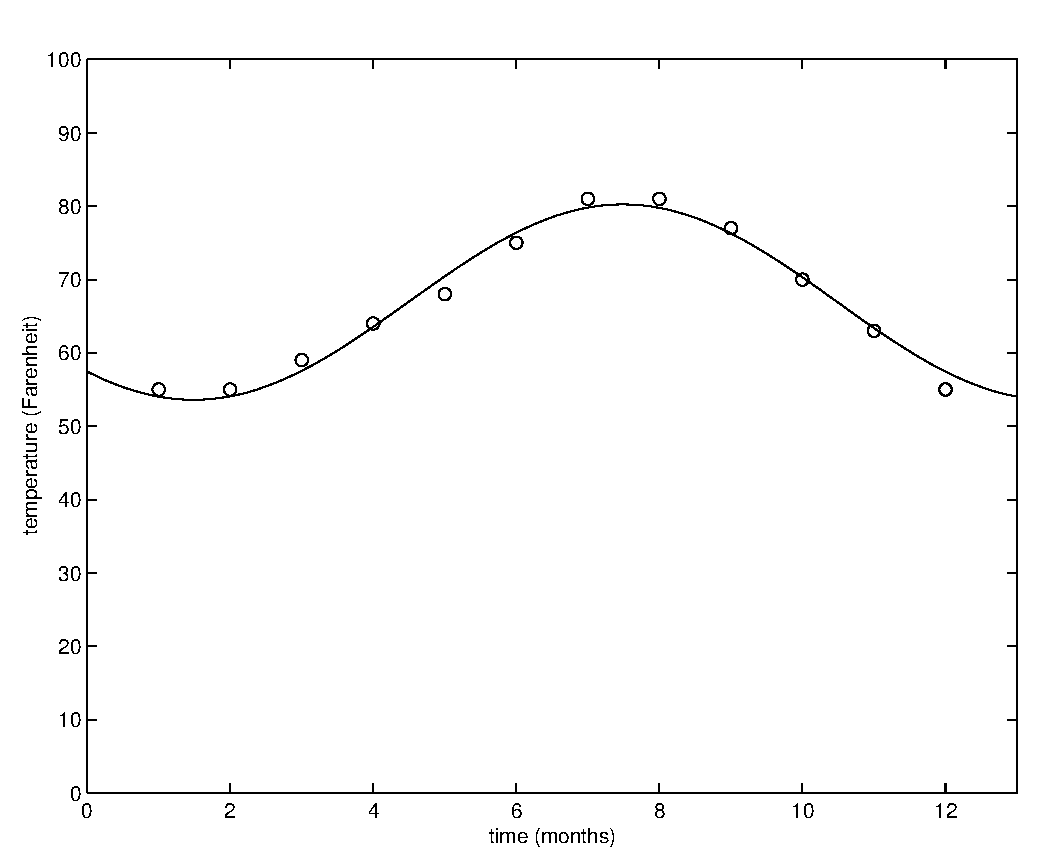
\psfig{file=../figures/ParisH.eps,width=2.5in}
     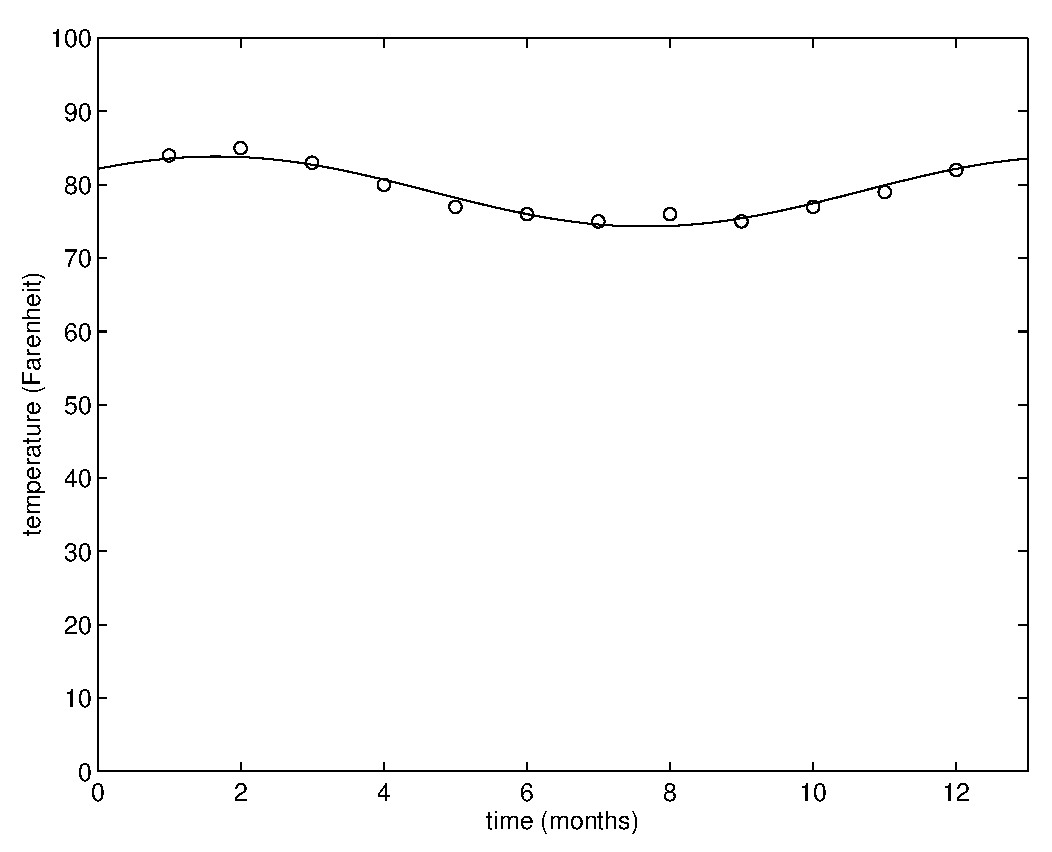
\psfig{file=../figures/RioH.eps,width=2.5in}}
     \caption{Monthly averages of daily high temperatures in Paris (left) and
	Rio de Janeiro (right) with best sinusoidal approximation.}
     \label{F:ParisH}
\end{figure*}

A similar exercise allows us to compute the best approximation to the
Rio de Janeiro high temperatures obtaining
\begin{verbatim}
b(1) =  79.0833
b(2) =   3.0877
b(3) =   3.6487
\end{verbatim}
The value of $b(1)$ is just the mean high temperature and not surprisingly
that value is much higher in Rio than in Paris.  There is yet more
information contained in these approximations.   For
the high temperatures in Paris and Rio
\[
d_P = 13.3244 \AND d_R = 4.7798.
\]
The amplitude $d$ measures the variation of the high temperature about its
mean.  It is much greater in Paris than in Rio, indicating that the
difference in temperature between winter and summer is much greater in Paris
than in Rio.

\subsubsection*{Least Squares Fit in \Matlabp}

The general formula for a least squares fit of data \eqref{E:LSFG} has been
preprogrammed in \Matlabp.  After setting up the matrix $A$ whose columns are 
the vectors $F_j$ just type
\begin{verbatim}
b = A\Y
\end{verbatim}
This \Matlab command can be checked on the sinusoidal fit to the high 
temperature Rio de Janeiro data by typing
\begin{verbatim}
b = A\RioH
\end{verbatim} 
and obtaining
\begin{verbatim}
b =
   79.0833
    3.0877
    3.6487
\end{verbatim}


\EXER

\includeexercises


\end{document}

%%% Local Variables:
%%% mode: latex
%%% TeX-master: "../linearAlgebra"
%%% End:
